\documentclass{article}

\usepackage{tabularx}
\usepackage{pdfpages}
% if you need to pass options to natbib, use, e.g.:
%     \PassOptionsToPackage{numbers, compress}{natbib}
% before loading neurips_2022


% ready for submission
%\usepackage{setup/neurips_2022}


% to compile a preprint version, e.g., for submission to arXiv, add add the
% [preprint] option:
\usepackage[preprint]{setup/neurips_2022}


% to compile a camera-ready version, add the [final] option, e.g.:
%     \usepackage[final]{setup/neurips_2022}


% to avoid loading the natbib package, add option nonatbib:
%    \usepackage[nonatbib]{setup/neurips_2022}


\usepackage[utf8]{inputenc} % allow utf-8 input
\usepackage[T1]{fontenc}    % use 8-bit T1 fonts
\usepackage{hyperref}       % hyperlinks
\usepackage{url}            % simple URL typesetting
\usepackage{booktabs}       % professional-quality tables
\usepackage{amsfonts}       % blackboard math symbols
\usepackage{nicefrac}       % compact symbols for 1/2, etc.
\usepackage{microtype}      % microtypography
\usepackage{xcolor}         % colors


% The \author macro works with any number of authors. There are two commands
% used to separate the names and addresses of multiple authors: \And and \AND.
%
% Using \And between authors leaves it to LaTeX to determine where to break the
% lines. Using \AND forces a line break at that point. So, if LaTeX puts 3 of 4
% authors names on the first line, and the last on the second line, try using
% \AND instead of \And before the third author name.


\author{
  Shao-Ting Chiu\thanks{UIN: 433002162} \\
  Department of Electrical and Computer Engineering\\
  Texas A\&M University\\
  College Station, TX 77843 \\
  \texttt{stchiu@tamu.edu} \\
  \AND
  Chan-Min Hsu\thanks{UIN: 532008407} \\
  Department of Electrical and Computer Engineering\\
  Texas A\&M University\\
  College Station, TX 77843 \\
  \texttt{chanminhsu@tamu.edu} \\
}

% Renumbering the supplemental materials
\newcommand{\beginsupplement}{%
        \setcounter{table}{0}
        \renewcommand{\thetable}{S\arabic{table}}%
        \setcounter{figure}{0}
        \renewcommand{\thefigure}{S\arabic{figure}}%
        \setcounter{section}{0}
        \renewcommand{\thesection}{S\arabic{section}}%
        \setcounter{equation}{0}
        \renewcommand{\theequation}{S\arabic{equation}}%
     }

\title{Predicting Stock Market with Bayesian Neural Network}


\begin{document}

\maketitle


\begin{abstract}
The randomness of the stock market challenge investments to be reliable. Many approaches have been introduced to find the hidden pattern behind the transitions. However, error estimation with the non-parametric method is in the early stage. In this project, we used a Bayesian neural network to predict discrete  time-series data with Taken's embedding theorem. In this project, The Unadjusted Langevin Monte Carlo, Metropolis-adjusted Langevin algorithm (MALA) and Hamiltonian Monte Carlo (HMC) are applied to measure the posterior distribution. We found that Langevin method performed best for the log likelihood optimization. The purpose of this project is to provide a model-free approach with uncertainty quantification that is essential to the investment strategy. 
\end{abstract}

\section{Introduction}


% Describe the goal of the project briefly, the data set, and the pattern recognition techniques to be used (e.g., data cleaning, data visualization/exploration, feature selection/extraction, classification/regression method, model selection, and error estimation).


% Dataset Bayesian neural network
% Things to write: Feedforward Neural Network with Parallel Tempering MCMC
% Dataset : time-series

Bayesian learning offers an intuitive method to estimate uncertainty and parameter quantification that is crucial for the stock market.  In this project, we reimplemented the Bayesian neural network to predict the stock price before and after COVID-19 prevalence \citep{chandra2021bayesian}. 

% With Bayesian learning first introduced to neural networks recently, it provides better model uncertainty quantification compared to classical neural networks.

%Our goal is to combine the Bayesian neural network with different techniques such as autoregressive integrated moving average (ARIMA) \citep{Rathnayaka2015AHS}. Furthermore, to accelerate the overall prediction time, we can adopt the an automatic differential equation with delay DE.


The impact of COVID-19 spreading on the stock price of a company in a country is predicted via Bayesian neural network with parallel tempering MCMC sampling\citep{chandra2021bayesian, chandra2019langevin} with uncertainty estimation. In \cite{chandra2021bayesian}, the prediction is made by the historical stock prices of a given country, which loses the information from other countries impacted by COVID-19 earlier. 
%Also,\href{https://twiecki.io/blog/2018/08/13/hierarchical_bayesian_neural_network/}{the hierarchical Bayesian method} provides an intuitive approach for pooling nested data, and allows group information to be shared and formulate a general model. 

\paragraph{Our goal} is to apply alternative sampling methods, such as Langevin MCMC or Hamiltonian MCMC, other than \citep{chandra2019langevin}, and predict the time-series data with Bayesian neural network. The pooled Bayesian neural network will be used as the informative prior of the target market stock. On the other hand, we introduce the just-in-time compilation (JIT), and automatic differentiation for Langevin Monte Carlo approaches with \textit{JAX}\citep{jax2018github} to compare the original method built by \textit{NumPy} and \textit{Multiprocessing}\citep{chandra2021bayesian}. %In the end, four in-group Bayesian neural networks will be marginalized via within-group data and combined into a global model. Noted that each framework can achieve its own task, but the information is shared with each group. The hierarchical Bayesian approach can overcome \href{https://www.pnas.org/doi/10.1073/pnas.1611835114#sec-3}{catastrophic forgetting in the neural networks} (old weights get overwritten) by sharing the higher-order representation informed by groups of data, and potentially improve prediction with augmented information.



\section{Methods}


\subsection{Dataset}

The stock dataset contains the closing price per day for 4 stocks in 4 countries (Table \ref{tab:my_label}). These discrete time-series data is processed by normalization ($x_{i}' = \frac{x_{i} - x_{\min}}{x_{\max} - x_{\min}}$). The dataset is labeled by two timeframes: before and during COVID-19 (Fig. \ref{fig:data-series}). Suppose the closing stock price is $[x_1, \dots, x_N]$ where $N$ is the length of the time series. The purpose is to predict the time series (prediction horizon) after the first few days (capture window).



The original data set is $x_t = \{x_{1}, ..., x_{Total}\}$, the training input is a matrix with dimension $m \times s$ (where m is the capture window, and $s$ is the number of samples). The sample is produced by shifting the original time series with a lag of $2$.  These discrete time-series data is processed by normalization ($x_{i}' = \frac{x_{i} - x_{\min}}{x_{\max} - x_{\min}}$). 

In this project, we used \textsc{MMM8} training set (Fig. \ref{fig:mm8-train}) for testing multiple Monte Carlo sampling methods for approximating the posterior distribution.

\begin{equation}
\bar{x}_t = 
\underbrace{\begin{bmatrix}
    x_{1+(t-1)T} & \cdots & x_{m+(t-1)T}\\
    x_{3+(t-1)T} & \cdots & x_{m+3+(t-1)T}\\
    \vdots & \vdots & \vdots 
\end{bmatrix}}_{\text{m (Capture windows)}}
\label{eq:window}
\end{equation}

\begin{equation}
y_t = 
\underbrace{\begin{bmatrix}
    x_{m+(t-1)T + 1} & \cdots & x_{m+(t-1)T+ n}\\
    x_{m+3+(t-1)T + 1} & \cdots & x_{m+3+(t-1)T+ n}\\
    \vdots & \vdots & \vdots
\end{bmatrix}}_{\text{n (Prediction Horizons)}}
\label{eq:ywindow}
\end{equation}


\begin{figure}[h]
     \centering
     \begin{subfigure}[b]{0.5\textwidth}
         \centering
         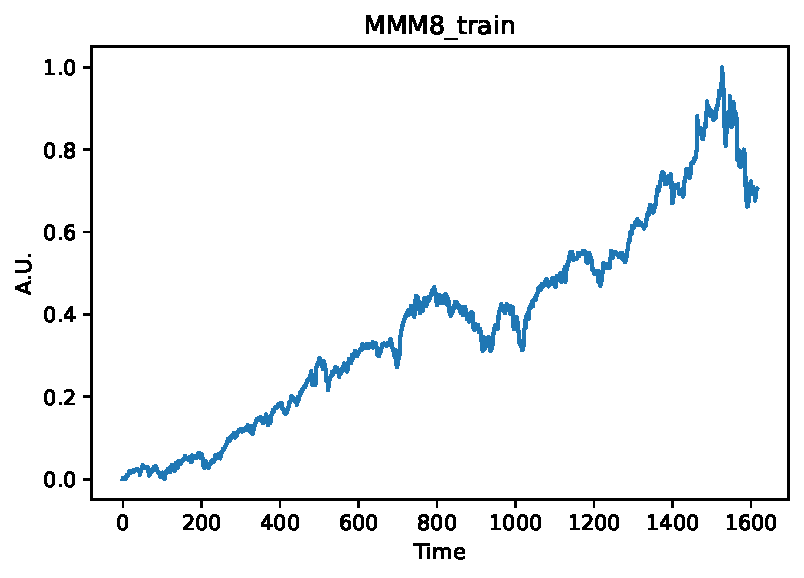
\includegraphics[width=\textwidth]{../img/MMM8_train.pdf}
         \caption{Train set (before COVID-19)}
         \label{fig:mm8-train}
     \end{subfigure}%
     \begin{subfigure}[b]{0.5\textwidth}
         \centering
         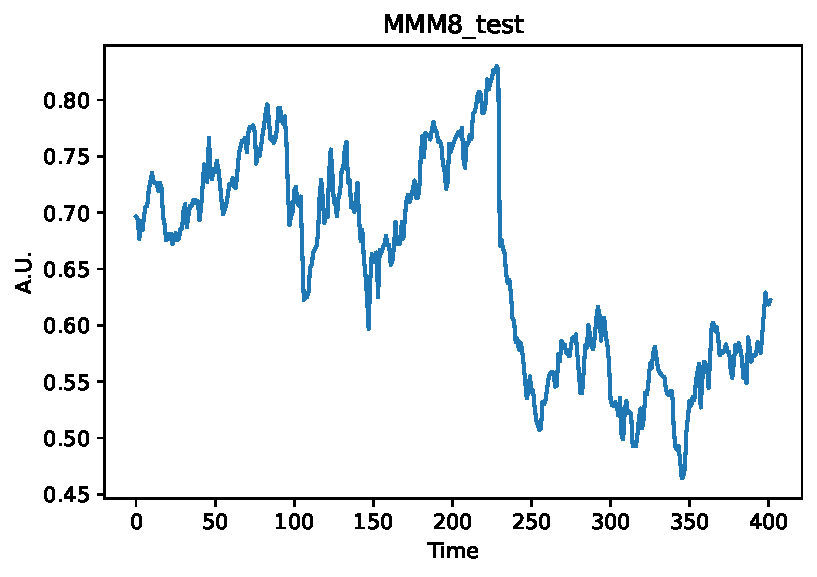
\includegraphics[width=\textwidth]{../img/MMM8_test.pdf}
         \caption{Test set (before COVID-19)}
     \end{subfigure}
     \hfill
     \begin{subfigure}[b]{0.5\textwidth}
         \centering
         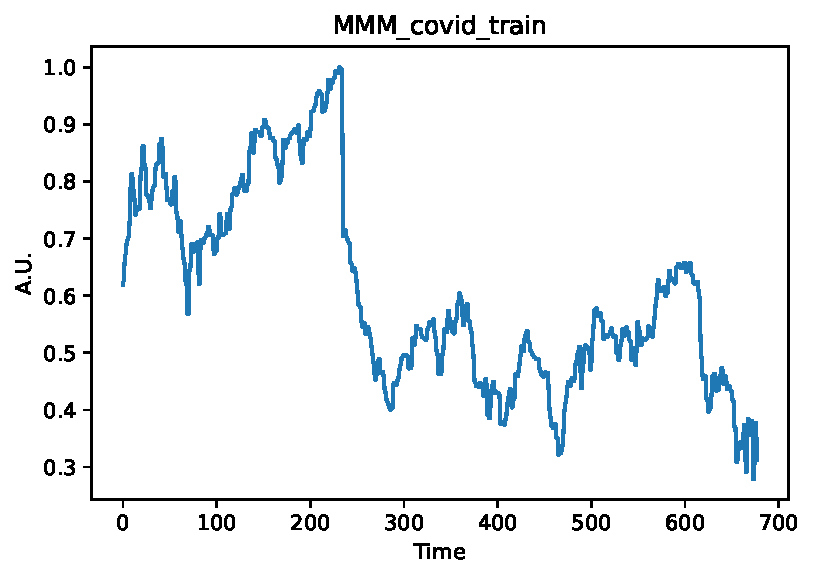
\includegraphics[width=\textwidth]{../img/MMM_covid_train.pdf}
         \caption{Train set during COVID-19}
     \end{subfigure}%
     \begin{subfigure}[b]{0.5\textwidth}
         \centering
         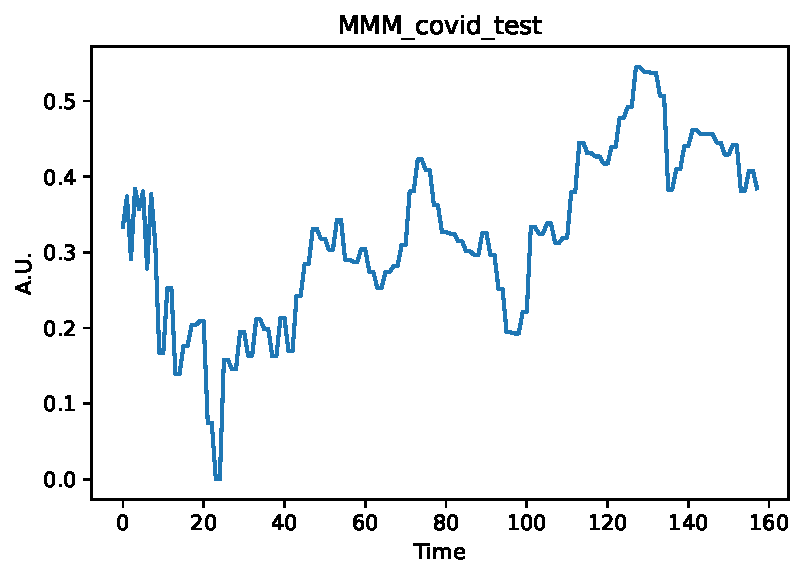
\includegraphics[width=\textwidth]{../img/MMM_covid_test.pdf}
         \caption{Test set during COVID-19}
     \end{subfigure}
    \caption{Stock markets of a company before and during COVID-19 \citep{chandra2021bayesian} (\href{https://github.com/stevengogogo/ECEN649_FinalProject/blob/main/script/EXP_data_visualization.ipynb}{source code}). The training set and testing set is recorded from the different time frame. The objective of \citep{chandra2021bayesian} is to fit each dataset with the same pipeline.}
    \label{fig:data-series}
\end{figure}


The state-space reconstruction is based on Taken's embedding theorem that guarantees the embedding time series (Eq. \ref{eq:window}) retains the manifold of the original dynamics\citep{takens1981detecting}.

\subsection{Framework}

The sequential neural network with one hidden layer is used for the regression problem. The activation function is $\tanh$\footnote{Notebooks and source code is provided at \url{https://github.com/stevengogogo/ECEN649_FinalProject}.}.

The implementation is based on \textit{Haiku} \citep{haiku2020github}, a neural network library with \textit{JAX} backend \citep{jax2018github}.


The input dimension is equal to the window size ($m$, Eq. \ref{eq:window}), and the output dimension corresponds to the prediction horizon ($n$, Eq. \ref{eq:ywindow}). The hidden layer contains 128 nodes. In practice, the properties of the Bayesian neural networks are saved with standard fixed-point neural networks and sampled parameters.


\subsection{Training}

The training process leverages the Bayes theorem (Eq. \ref{eq:bayes}):

\begin{equation}
P(\theta | D) \propto P(D|\theta) P(\theta)
\label{eq:bayes}
\end{equation}

where $\theta$ are parameters and $D$ is dataset. The prior distribution 

\begin{equation}
P(\theta) \sim Normal(0, \Sigma)
\label{eq:weight-prior}
\end{equation}


\subsection{Supervised Maximum likelihood learning}

The output of a neural network function is 

\begin{equation}
    \hat{y} = f(x, \theta)
    \label{eq:net-output}
\end{equation}

where $\theta$ is the random vector of weights of a neural network, $\hat{y}$ the predicted value, and $f$ the function of the neural network.

Because the weights ($\theta$) have Normal prior (Eq. \ref{eq:weight-prior}),  the likelihood of the target value ($y$) is 

\begin{equation}
    p(y|\hat{y}) = \frac{1}{\sqrt{2\pi}\sigma}e^{-\frac{(y-\hat{y})^2}{2\sigma^2}}
    \label{eq:likelihood}
\end{equation}

Thus, the likelihood is a Gaussian distribution with network output ($\hat{y}$) as a center. Eq. \ref{eq:likelihood} can be expressed in $\log$-form to avoid numerical instability of small values (Eq. \ref{eq:log-likelihood}).

\begin{equation}
    log (p(y|\hat{y})) = k + \frac{(y-\hat{y})^2}{2\sigma^2}
    \label{eq:log-likelihood}
\end{equation}


To find the most probable wight vector ($\theta$, Eq. \ref{eq:net-output}), the Maximum a Posteriori (MAP) is applied to \textit{maximize} the log-likelihood (Eq. \ref{eq:log-likelihood}). Because $\log$ (Eq. \ref{eq:likelihood}) is a monotonous function, the maximization of posterior can be achieved by maximizing the sum. From Eq. \ref{eq:bayes}, 

\begin{align}
    p(\theta|D) &= p(\theta) p(D|\theta) / p(D)\\
    \log(p(\theta|D)) &= \underbrace{\log(p(\theta))}_{\text{Log. prob. under prior}} + \underbrace{\log(p(D|\theta))}_{log. likelihood} - \underbrace{\log(p(D))}_{\text{log marginal probability of } D \text{(ignorable)}}\label{eq:log-sums}
\end{align}

The logarithm of posterior distribution is related to the log probability and log likelihood. Noted that the log marginal probability of $D$ is ignorable because it is a constant and independent of $\theta$. This ignorance can bypass the necessity of integration over the distribution.


Assuming data is independently and identical distributed (i.i.d.), the log-likelihood is computed by the product of the likelihood of all trials (Eq. \ref{eq:sum-log}).

\begin{equation}
    P(D|\theta) = \prod_{i\in \mathbb{D}} p(y_i | \theta) = \prod_{i \in \mathbb{D}} p(y_i | f(x, \theta))
\label{eq:sum-log}
\end{equation}

where $D$ is the sampled dataset from sample space $\mathbb{D}$. From Eq. \ref{eq:log-sums} and Eq. \ref{eq:sum-log}, the maximization of posterior distribution can be done by looking for right setting of prior and calculating likelihood. The posterior probability can be further simplified if the output is a Gaussian process (Sec. \ref{sec:gaus-pred}). However, the full posterior distribution over all parameters can not be easily derived, the Monte Carlo sampling method is applied to generate sample to approximate the posterior density function. 

\subsection{Approximation of Posterior Distribution by Monte Carlo Approaches}

Because there is no closed form of the posterior distribution, a Metropolis-adjusted Langevin algorithm (MALA)\citep{roberts1998optimal}, Unadjusted Langevin Algorithm\citep{durmus2019high} and Hamiltonian Monte Carlo\citep{neal1996} are applied to approximate the posterior probability density, and the gradient of probability is calculated via automatic differentiation. The Langevin algorithm provides a better acceptance rate compared to the naive Metropolis-hasting algorithm\citep{roberts1998optimal}. 

The sampling process is divided into three steps:

\begin{enumerate}
    \item \textbf{Initiation} The initiation step uses the prior distribution to sample initial parameters.
    \item \textbf{Proposal} The proposed step uses proposal distribution to generate a  parameter set. This step is optimized by a variety of approaches\citep{jospin2022a}: Hamiltonian Monte Carlo\citep{neal1996, neal2011}, MALA, and other gradient-based methods provide \textit{smart} sampling to yield better mixing and acceptance rate. These approaches are available at \textit{jax-bayes} package\footnote{https://github.com/jamesvuc/jax-bayes}. In MALA, the stochastic differential equation is solved to generate a new state. This approach is inspired by the physical diffusion and has an optimal acceptance rate $0.574$\citep{roberts1998optimal}.
    \item \textbf{Update} The generated sample is decided to accept or reject with the ratio of the probability of current and proposed states. Though the ratio is measured with different methods, the purpose is to avoid integrating the marginal probability of posterior distribution.
\end{enumerate}


The log-likelihood is used to avoid numerical instability when encountering small numbers. In practical (Fig. \ref{fig:training-log}), the log-likelihood can be $10^{-14}$. 

\subsection{Difference from the \citep{chandra2021bayesian}}

In \cite{chandra2021bayesian}, the parallel tempering method is used to train the Bayesian neural network. The source code of \citep{chandra2019langevin} is implemented by NumPy and Multiprocessing. In this project, we are exploring one or several sampling methods and leveraging the just-in-time compilation (JIT) powered by JAX\citep{jax2018github}. The sampling process is compiled to machine code and can be moved to hardware acceleration such as GPU/TPU.



\section{Results}

\subsection{Suboptimal training with MALA}

The iteration of $5\times 10^4$ is used to derive the posterior distribution. Each iteration yields $30$ samples to calculate the log-likelihood. The training log (Fig. \ref{fig:training-log}) shows that more iteration is needed to achieve a higher log-likelihood. 

\begin{figure}[h]
    \centering
    \begin{subfigure}[b]{0.5\textwidth}
        \centering
        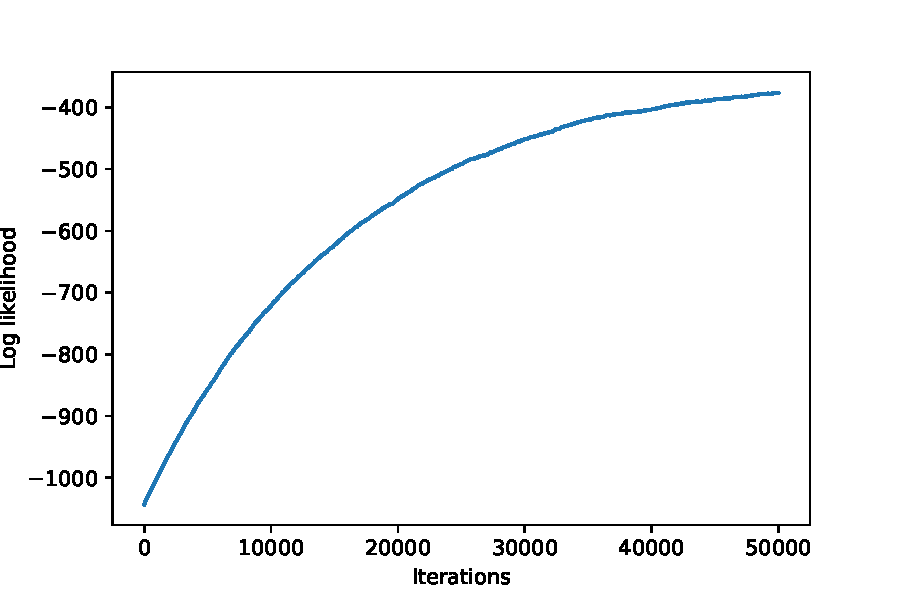
\includegraphics[width=\textwidth]{../img/training_MALA_50000-iter.pdf}
        \caption{Training loss (likelihood).}
        \label{fig:training-log}
    \end{subfigure}%
    \begin{subfigure}[b]{0.5\textwidth}
        \centering
        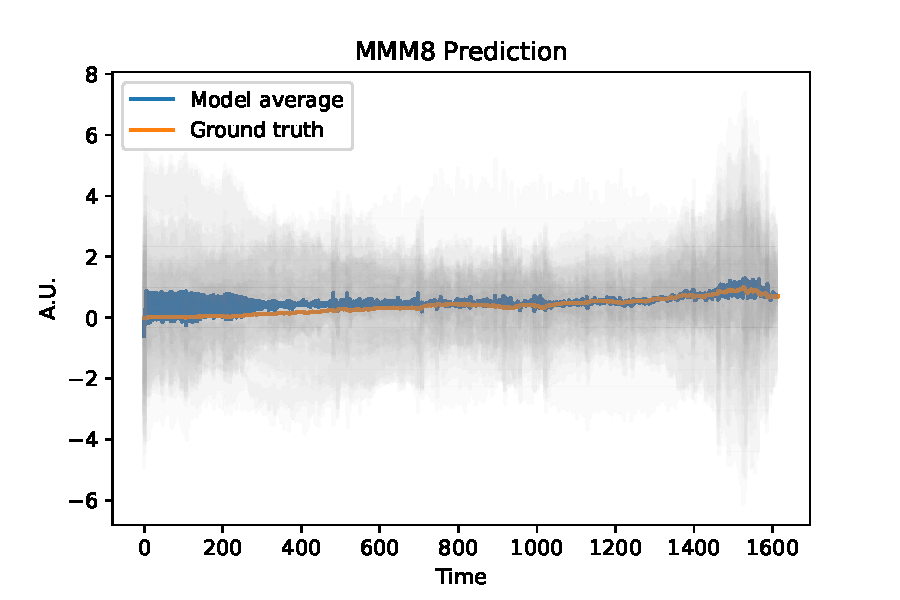
\includegraphics[width=\textwidth]{../img/prediction_MALA_50000-iter.pdf}
        \caption{Prediction (training set)}
        \label{fig:pred-sub}
    \end{subfigure}
    \caption{Training with MALA method\citep{roberts1998optimal}. The training process took $30$ min on MacPro M1 Chip. (b) Prediction is made by sampling $30$ times. Each time series is plotted in semi-transparent gray. The mean and ground truth are plotted, respectively. (See Sec. \ref{sec:notebook} for implementation details.)}
    \label{fig:pred}
\end{figure}

\subsection{Suboptimal training with Langevin}

The iteration of $2\times 10^5$ is used to derive the posterior distribution. Each iteration yields $30$ samples to calculate the log-likelihood. The training log (Fig. \ref{fig:training-log-lagevin}) reaches the optimal value of log-likelihood after $2\times 10^5$ times. Noted that the performance is better when choosing sigmoid function as our activation function than tanh function (Fig. \ref{fig:prediction-sigmoid}, \ref{fig:prediction-tanh}).

\begin{figure}[h]
    \centering
    \begin{subfigure}[b]{0.5\textwidth}
        \centering
        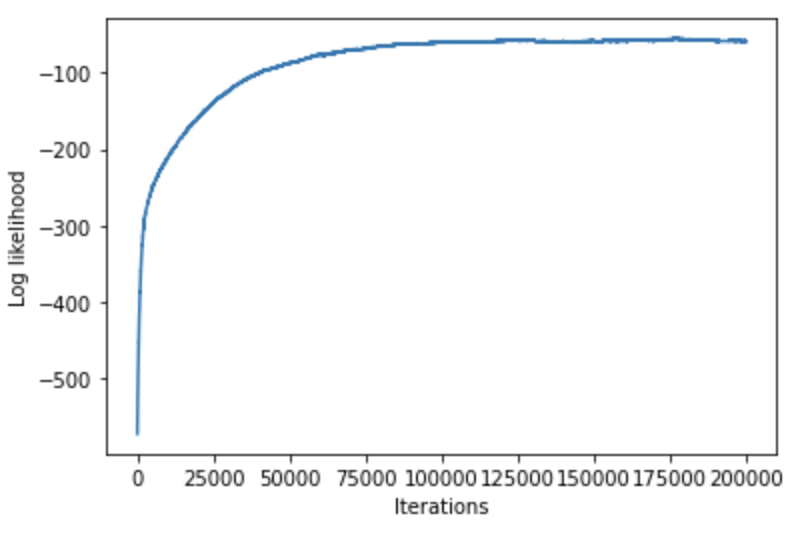
\includegraphics[width=\textwidth]{../img/training_Langevin_200000_iter.png}
        \caption{Training log of sigmoid activation}
        \label{fig:training-log-lagevin}
    \end{subfigure}\hfill
    \begin{subfigure}[b]{0.5\textwidth}
        \centering
        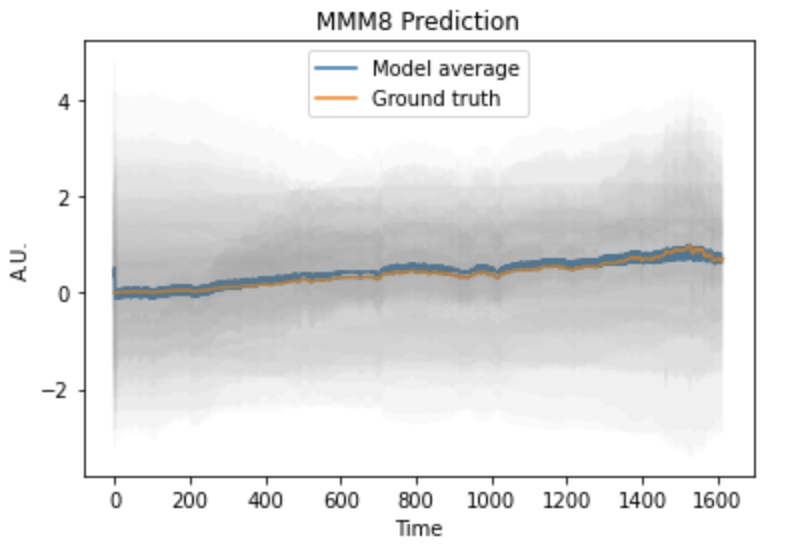
\includegraphics[trim={0 0 0 0.7cm}, clip, width=\textwidth]{../img/prediction_Langevin_200000_iter.png}
        \caption{Prediction of sigmoid activation}
        \label{fig:prediction-sigmoid}
    \end{subfigure}
    \begin{subfigure}[b]{0.5\textwidth}
        \centering
        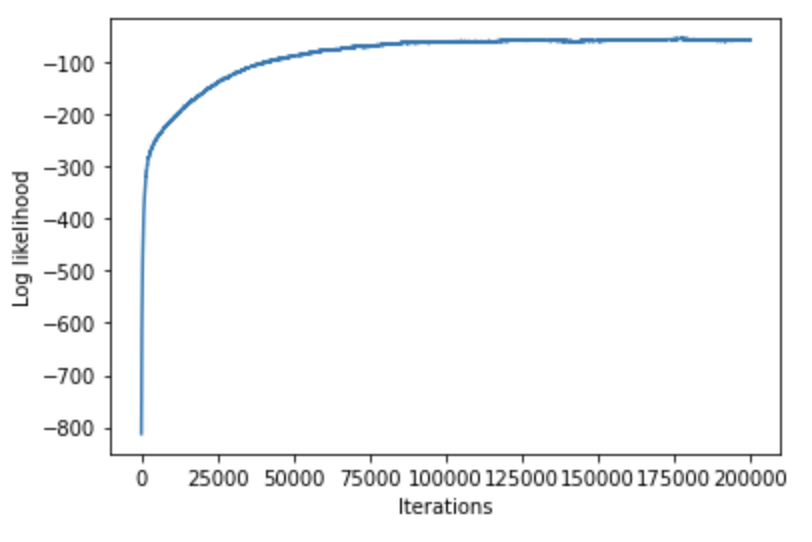
\includegraphics[width=\textwidth]{../img/training_Langevin_200000_tanh.png}
        \caption{Training log of tanh activation}
    \end{subfigure}\hfill
    \begin{subfigure}[b]{0.5\textwidth}
        \centering
        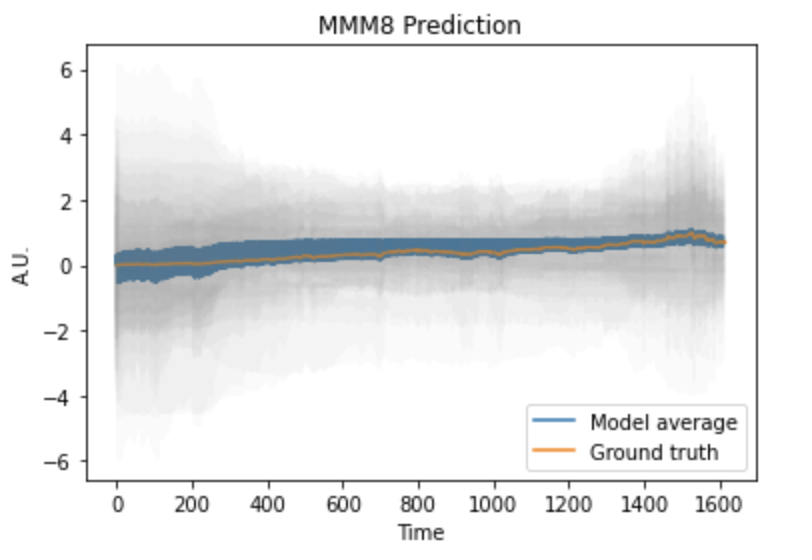
\includegraphics[trim={0 0 0 0.7cm}, clip, width=\textwidth]{../img/prediction_Langevin_200000_tanh.png}
        \caption{Prediction of tanh activation}
        \label{fig:prediction-tanh}
    \end{subfigure}
    \caption{Training with Unadjusted Langevin Method\citep{durmus2019high}. The training process took $45$ min on MacPro Intel i5 Chip. (b)(d) Prediction is made by sampling $30$ times. Each time series is plotted in semi-transparent gray. The mean and ground truth are plotted, respectively.}
\end{figure}


\subsection{HMC failed to find the posterior distribution}

The iteration of $4\times 10^5$ is used to derive the posterior distribution. Each iteration yields $30$ samples to calculate the log-likelihood. Same as MALA method, more iteration is needed to achieve a higher log-likelihood (Fig. \ref{training-log-HMC}). Noted that the prediction of HMC (Fig. \ref{prediction-HMC})is more noisy compared to other methods.

\begin{figure}[h]
    \centering
    \begin{subfigure}[b]{0.5\textwidth}
        \centering
        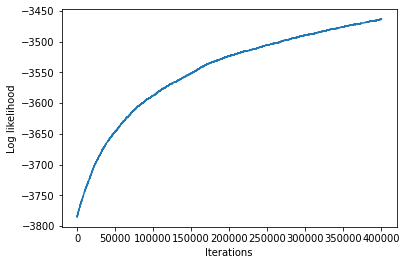
\includegraphics[width=\textwidth]{../img/training_HMC_400000_iter.png}
        \caption{Training log of sigmoid activation}
        \label{training-log-HMC}
    \end{subfigure}\hfill
    \begin{subfigure}[b]{0.5\textwidth}
        \centering
        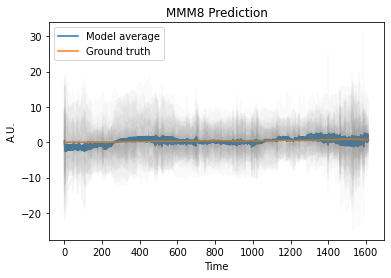
\includegraphics[trim={0 0 0 0.7cm}, clip, width=\textwidth]{../img/prediction_HMC_400000_iter.png}
        \caption{Prediction of sigmoid activation}
        \label{prediction-HMC}
    \end{subfigure}
    \caption{Training with Hamiltonian Monte Carlo Sampling\citep{neal1996}.}
\end{figure}

\subsection{With sampling method fixed, model size is not proportional to log likelihood.}

The model size is not proportional to the log likelihood. In Fig. \ref{fig:big-net-training}, the model with hidden layer of 128 nodes performs worse than the model with hidden layer of 10 nodes. This implies that the complicated neural network does not always lead to better result, which is similar to the scissor effect \citep[Ch 1.]{braga2020fundamentals}.
 
\begin{figure}[h]
    \begin{subfigure}[b]{0.5\textwidth}
        \centering
        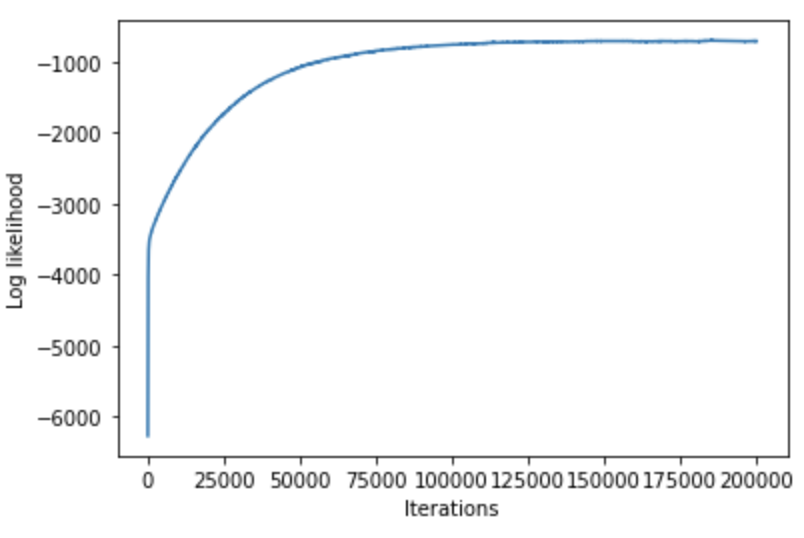
\includegraphics[width=\textwidth]{../img/training_Langevin_200000_128.png}
        \caption{Training with Langevin Monte Carlo Sampling}
        \label{fig:big-net-training}
    \end{subfigure}\hfill
    \begin{subfigure}[b]{0.5\textwidth}
        \centering
        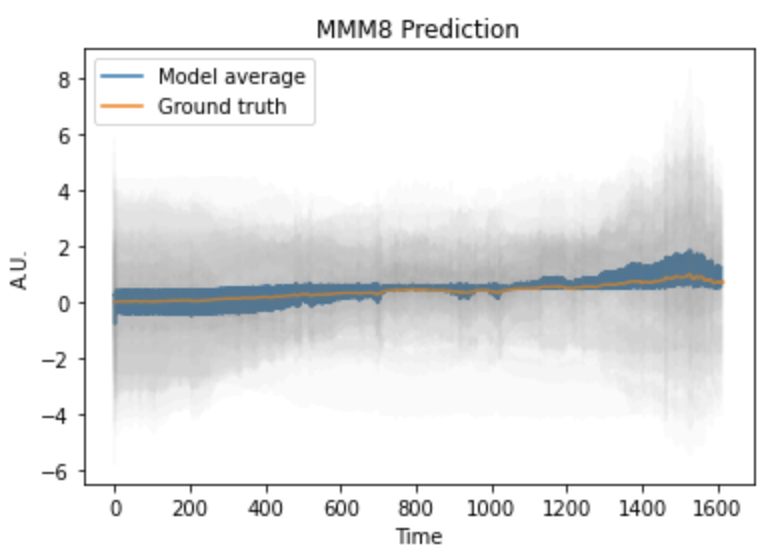
\includegraphics[trim={0 0 0 0.7cm}, clip, width=\textwidth]{../img/prediction_Langevin_200000_128.png}
        \caption{Prediction with Langevin Monte Carlo Sampling}
    \end{subfigure}
    \caption{Training with neural network with hidden layer of 128 nodes.}
\end{figure}

\section{Discussion}

\subsection{Langevin methods provide better posterior approximation of high dimensional Bayesian neural network than Hamiltonian Monte Carlo}

The Hamiltonian Monte Carlo is a classic sampling method for Bayesian neural network\citep{neal1996}, that is inspired by the Hamiltonian mechanics. In pratical, this method requires fine-tuning of two parameters: leapfrog step and iterations. As shown in Fig. \ref{training-log-HMC}, the log likelihood is poorly found. This may due to ill-defined parameter setting of leapfrog and sampling iterations, and finding appropriate parameter setting is the difficult part of Hamiltonian Monte Carlo. Notebly, No-U-Turn sampler modified HMC and does not require the parameter tuning\citep{hoffman2014no}. The Langevin method seems more suitable for this model (Fig. \ref{fig:training-log-lagevin}) with the proposed setting (Sec. \ref{sec:notebook}). However, the solid conclusion requires the exploration of parameter setting of leapfrog and iterations.


\subsection{Token's embedding method introduces correlation in dataset }

In \cite{chandra2021bayesian}, the log likelihood is applied to find the best distribution of posterior. The likelihood $p(D|\theta)$ is the product of all i.i.d. experiments (Eq, \ref{eq:likelihood}). The autocorrelation is one concerned when applying log likelihood (Eq. \ref{eq:log-likelihood}). As shown in Fig. \ref{fig:auto}, the stock market signal is autocorrelated, and that introduces correlation in dataset matrix (Eq. \ref{eq:window}). In the case of correlated sampling of $x$, the log likelihood may not be simply the product of all trials. The violated i.i.d. assumption can change the posterior distribution, and the correlation problem is not discussed in \cite{chandra2021bayesian}.

\subsection{Jax implementation provides compiled script and hardware acceleration compared to the original implementation}

Inspired by the source code of \cite{chandra2021bayesian}, we leveraged the acceleration of Jax library \citep{jax2018github}. In Sec. \ref{sec:notebook}, the \textit{@jax.jit} decorator can convert the python function into compiled machine code and speed up the for-loop (more example are shown in Sec. \ref{sec:notebook}). On the other hand, the automatic differential equation is another advantage to use Jax, that produces differential type of function from the customized function. This feature is essential for the speed of gradient-based sampling that used in this project. 

The source code of \cite{chandra2021bayesian} is coded in \textit{NumPy} and \textit{Multiprocessing}. This setting is limited to the parallel processing in CPU. The Jax implementation enables the hardware acceleration via GPU/TPU. The GPU acceleration via \textit{NVIDIA Tesla T4} roughly provides three times acceleration compared to training on single core CPU. Though the re-implementation provides heuristic trials of Unadjusted Langevin, MALA and HMC, the novel multiple tempering method proposed \citep{chandra2019langevin} is not tested as reference.

\cite{chandra2021bayesian} uses $10000$ sample number to generate the result, and the sampling method tried in this project requires 10 times of iterations. This shows that the proper design of sampler is crucial for Bayesian neural network approach.





\begin{figure}[htb]
    \centering
    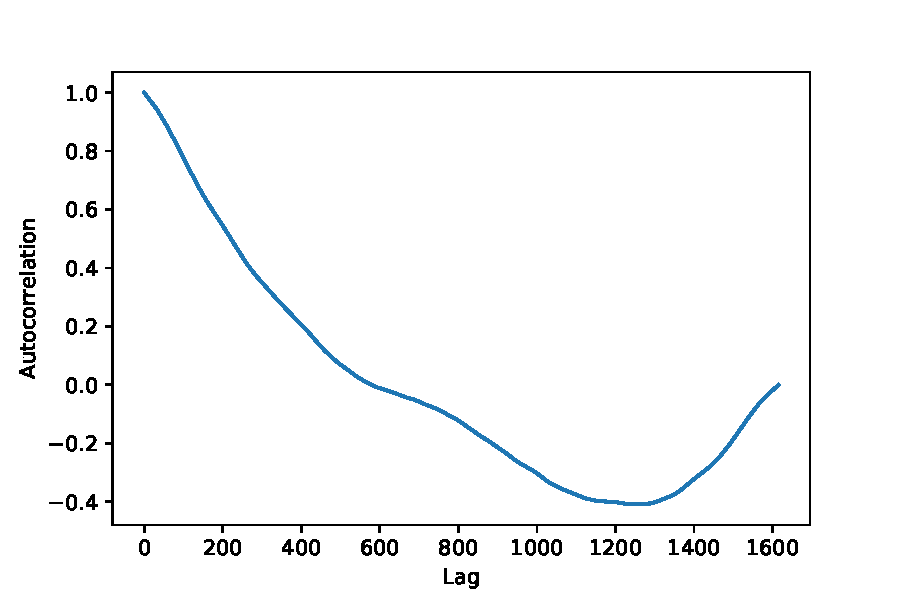
\includegraphics[width=0.7\textwidth]{../img/autocorrelation.pdf}
    \caption{Autocorrelation of the stock market signal (Fig. \ref{fig:mm8-train})}
    \label{fig:auto}
\end{figure}


\bibliography{ref}

\beginsupplement
\section{Supplemental Materials}

\subsection{Github Repositories and Dataset}

\begin{table}[h]
    \centering
    \begin{tabularx}{\textwidth}{cX}
       \textbf{Resources} & \textbf{Description} \\
       \hline
       \href{https://github.com/sydney-machine-learning/Bayesianneuralnet_stockmarket}{Source code  of \citep{chandra2021bayesian}} & See primary paper\citep{chandra2021bayesian}. This paper applied langevin-gradient parallel tempering from \citep{chandra2019langevin} with stock data under the influences of COVID-19\\\hline
       \href{https://github.com/sydney-machine-learning/parallel-tempering-neural-net}{Source code of \citep{chandra2019langevin}} & See secondary paper\citep{chandra2019langevin} that propose parallel computing of langevin gradient Monte Carlo for Bayesian neural network\\\hline
        \href{https://github.com/sydney-machine-learning/Bayesianneuralnet_stockmarket/blob/master/code/datasets/raw/DAI.DE.csv}{Raw data}  & The original dataset with opened, closed, highest, lowest prices within a day. 1267 days recorded.  \\\hline
       \href{https://github.com/sydney-machine-learning/Bayesianneuralnet_stockmarket/blob/master/code/datasets/600118.SS_1_train.txt}{Processed dataset}  & Filtered dataset. In \cite{chandra2021bayesian}, only one feature is used per day. Noted that the data is non-stationary  \\\hline
       \href{https://github.com/sydney-machine-learning/Bayesianneuralnet_stockmarket/blob/6d24cf25115b6517e3099249bc657674f6b9b98f/code/pt_timeseries_regression.py\#L36-L142}{Bayesian framework} & The implementation is based on \texttt{NumPy}, and the parallel tempering is based on \texttt{multiprocess} package. The computation requires multiprocessing with CPUs.\\\hline
       \href{https://github.com/jamesvuc/jax-bayes}{Jax-Bayes} & Bayesian inference with Jax\citep{jax2018github}.\\\hline
       \href{https://github.com/stevengogogo/ECEN649_FinalProject}{ECEN649\_FinalProject} & Project code and documentation
    \end{tabularx}
    \caption{Resources table.}
    \label{tab:my_label}
\end{table}


\subsection{Log likelihood of Gaussian prediction\label{sec:gaus-pred}}

If the model produces Guassian prediction ($\hat{y} \sim Normal(\mu_D, \sigma^{2}_{D})$), Eq. \ref{eq:log-sums} can be inferred to 

\begin{equation}
    -\log(p(\theta |D)) = \frac{1}{2\sigma^{2}_{D}} \sum_{i \in \mathbb{D}}(\hat{y}_i - y_i) + \frac{1}{2\sigma^{2}_{\theta}} \sum_{i}\theta_{i}^{2}
\end{equation}


\subsection{Example Notebook\label{sec:notebook}}

The experiments are made and recorded in Jupyter notebooks. The following is an printout of an example that uses Langevin Monte Carlo for training the Bayesian neural network proposed in \cite{chandra2021bayesian}. This notebook is available on Google Colab\footnote{Notebook on Colab: \url{https://colab.research.google.com/drive/19yguqrHEPuBiJjGrUHsA5NMybO7q32RP?usp=sharing}} with GPU acceleration.


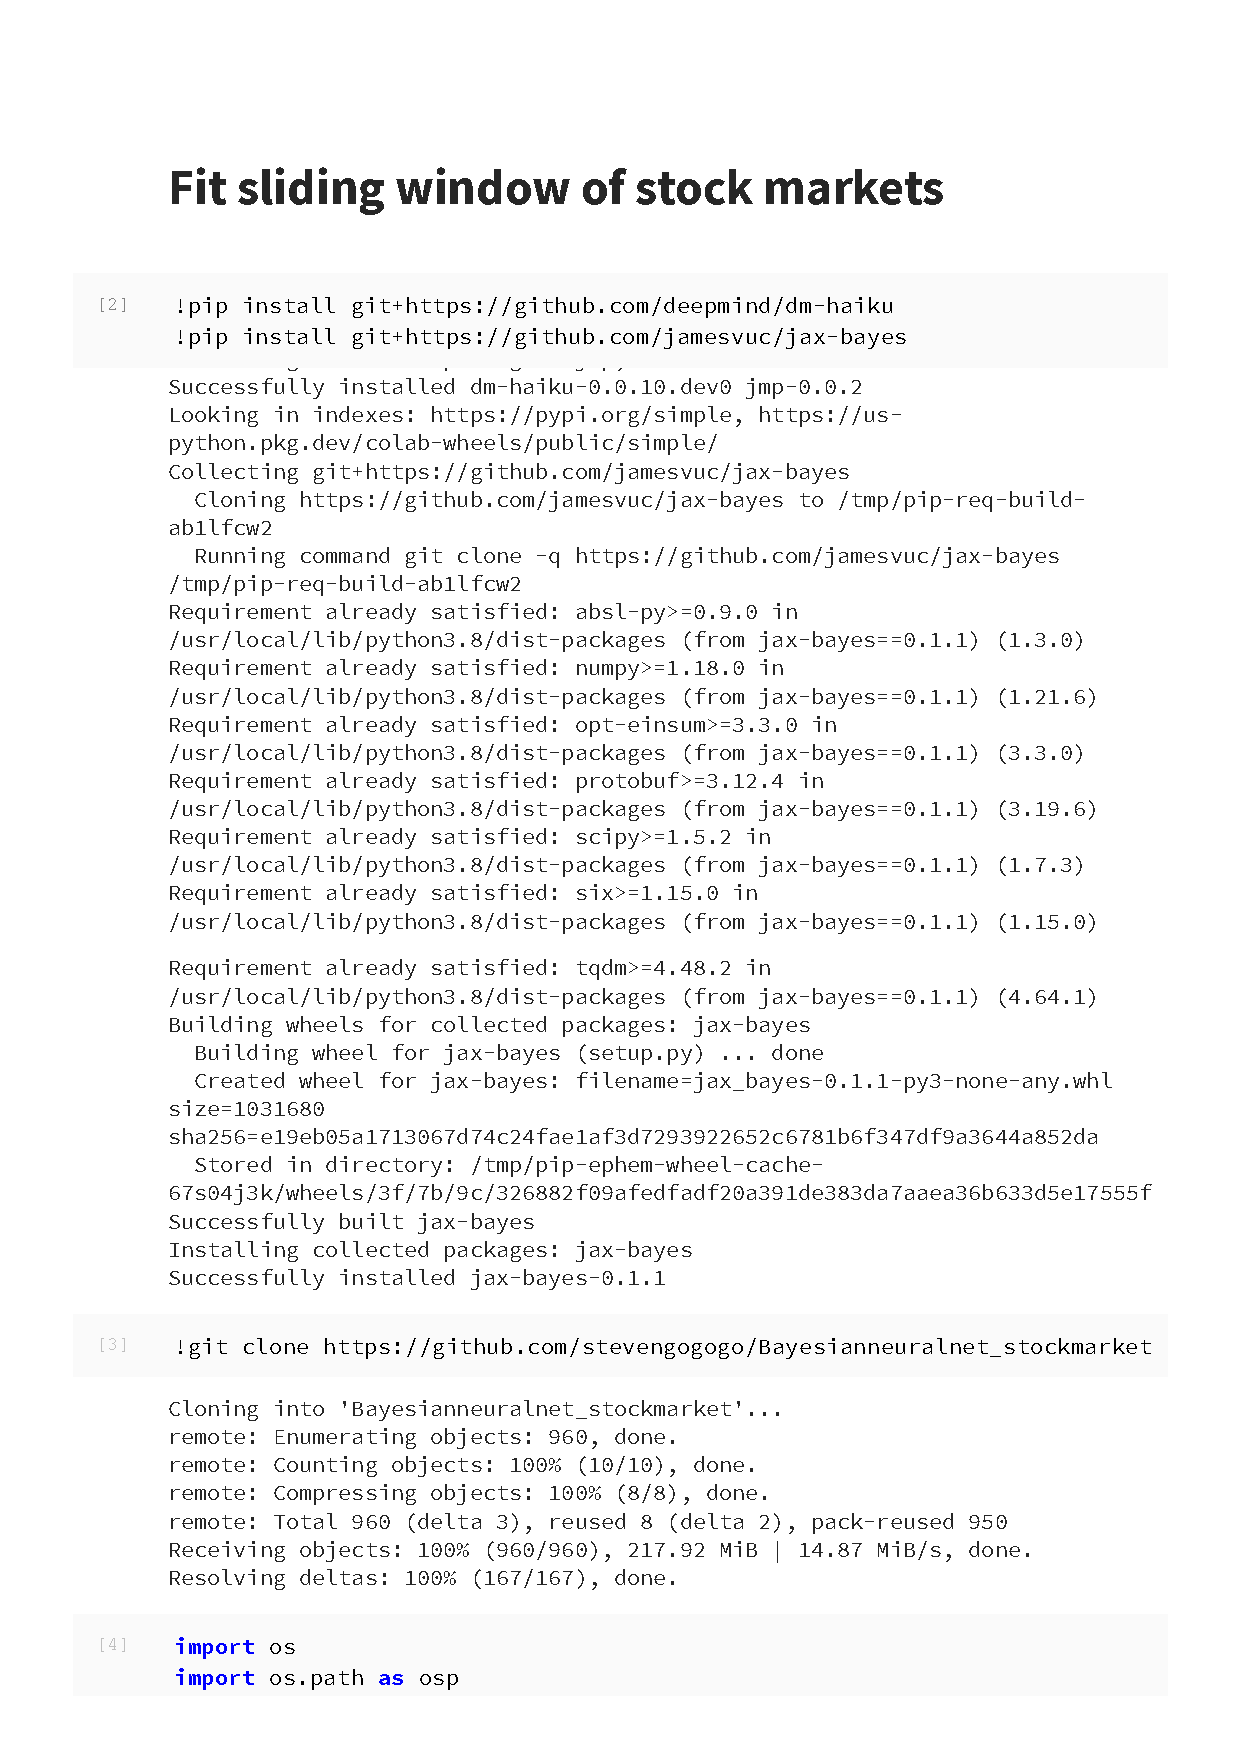
\includepdf[pages=-,width=\textwidth]{../img/Sigmoid_EXP_fit_time_window.pdf}

\end{document}